\section*{\fs{12}Tablica lekarstwa-recepty}
\par{
\fs{12}

\begin{figure}[h!]
    \centering
   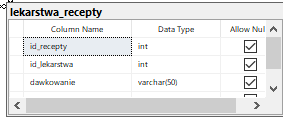
\includegraphics{Images/Zadanie2/lekarstwa_recepty.png}
    \caption{Tablica lekarstwa-recepty}
    \label{fig:my_label}
\end{figure}

\listsinglespacing{
\fs{12}
\begin{lstlisting}[frame=single,language=SQL,]
Select * from lekarstwa-recepty

\end{lstlisting}
\begin{figure}[h!]
    \centering
   \scalebox{.85}{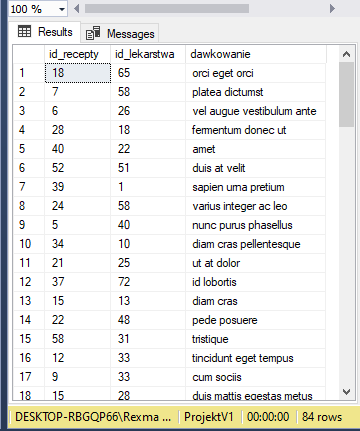
\includegraphics{Images/Zadanie2/Zapelnione/lekarstwa_recepty__query.png}}
    \caption{Wynik Zapytania}
    \label{fig:my_label}
\end{figure}
}